%% -*- mode: LaTeX -*-
%%

%%%%%%%%%%%%%%%%%%%%%%%%%%%%%%%%%%%%%%%%%%%%%%%%%%%%%%%%%%%%%%%%%%%%%%%%%%%%%%%

\section{Approach}
\label{sec:approach}

Our approach is designed towards using modified BGP at the control plane and segment Routing
at the data plane.  \textbf{Figure~\ref{fig:example3}} shows an example topology where AS1, AS2, 
and AS3 are three connected Autonomous systems. H-7 in AS1 has requested a data transfer to
H-16 in AS3. For the sake of this example lets assume that H-16's advertisement contains H-16's 
prefix, and a large BGP community attribute of the form 3:5:2. Thus, thanks to BGP, H-7 is made 
aware of H-16 and its attributes. BGP's large community attribute tells the ASes that come in 
contact with the advertisements that H-16's comes from AS3, and that we would like to associate
service 5, and of that service we would like type 2. To give a more concrete example lets associate 
service 5 with data transfers, and type 2 to be large elephant flows. Thus, H-16 would be associate
with large data flow transfers. When H-7 sends data to H-16, H-7's packets through the use of SDN
will be matched by destination and be prepended a segment routing header. The segment routing
header is formed by the service specific control unit. The service specific control unit is made aware
of BGP advertisements and associates paths within the AS to depending on the BGP large community
attribute that is being advertised. Next all traffic from H-7 to H-16 will be segment routed through AS1
and into AS2. AS2 has also established its own segment routing paths depending on the type of large
community attributes advertised by the prefix. Thus a new segment routing header is added at the 
gateway router to guide the packets to their destination. 

We will now go more into detail behind the specifics of our approach.

\textbf{BGP:} This component in our design handles the control plane. The prefixes advertised by an AS
reaches all connected ASes through the use of iBGP and eBGP. Furthermore, each advertised prefix
contains a large community attribute. The large community attribute ties a prefix with a specific service
that will be acted upon by each AS. The BGP large community attribute~\cite{largeBGP} consists of
three 4-octet values. GlobalAdminstrator:Function:Parameter. The first 4-octet value refers to the global
administrator. In our approach the global administrator will represent the AS number. The remaining 
two 4-octet values will represent the service and the type. Services can be any type of internet traffic
(e.g. data transfer, video streaming). While the type value is a specific type within the service (e.g 
for data transfer we could have large data transfers). The services associated with each large community
attribute will be an agreed upon policy between all ASes. 

\textbf{Service Specific Control Unit:} This component in our design is used to map control plane
BGP advertisements to appropriate segment routing paths. Using link state data the service specific 
control unit will automatically form segment routing headers that are used to guide the packet through
the AS based on the constraints associate with the advertisements large community attribute. 

\textbf{SDN:} This component in our design is primarily used to map a packet to an appropriate 
segment routing header. SDN will work closely with the service specific control unit to match 
a packet's destination, and prepend the segment routing header to the packet to guide it through 
the AS.
\begin{figure}
  \centering
  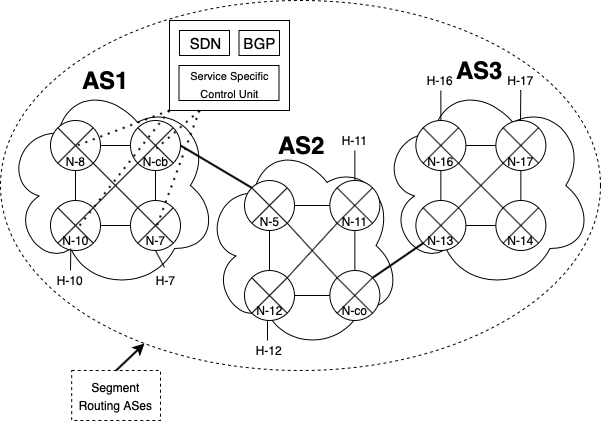
\includegraphics[width=0.9\columnwidth]{3ASFig}
  \caption{End to End Interdomain Example}
  \label{fig:example3}
\end{figure}




%%%%%%%%%%%%%%%%%%%%%%%%%%%%%%%%%%%%%%%%%%%%%%%%%%%%%%%%%%%%%%%%%%%%%%%%%%%%%%%

%% End of file.











































